\documentclass[11pt, letterpaper]{article}
\usepackage[utf8]{inputenc}
\usepackage[letterpaper, margin=0.5in]{geometry}
\usepackage{amsmath}
\usepackage{amssymb}
\usepackage{amsthm}
\usepackage{graphicx}
\usepackage{listings}
\usepackage[font=scriptsize]{caption}
\usepackage{subcaption}
\usepackage{xcolor}

\newtheorem{lemma}{Lemma}
\newcommand{\indep}{\perp \!\!\! \perp}

\definecolor{codegreen}{rgb}{0,0.6,0}
\definecolor{codegray}{rgb}{0.5,0.5,0.5}
\definecolor{codepurple}{rgb}{0.58,0,0.82}
\definecolor{backcolour}{rgb}{0.95,0.95,0.92}

\lstdefinestyle{mystyle}{
    backgroundcolor=\color{backcolour},   
    commentstyle=\color{codegreen},
    keywordstyle=\color{magenta},
    numberstyle=\tiny\color{codegray},
    stringstyle=\color{codepurple},
    basicstyle=\ttfamily\footnotesize,
    breakatwhitespace=false,
    texcl=true,
    mathescape=true,
    breaklines=true,                 
    captionpos=b,                    
    keepspaces=true,                 
    numbers=left,                    
    numbersep=5pt,                  
    showspaces=false,                
    showstringspaces=false,
    showtabs=false,                  
    tabsize=2
}

\lstset{style=mystyle}
\graphicspath{ {.} }
\captionsetup{justification=raggedright, singlelinecheck=false}

\author{Ryan Tang}
\title{STA 542 HW 2}
\date{March 2nd 2023}

\begin{document}
\maketitle

\section{Ex 1}
Suppose we know the underlying truth $Y = X^2 + Z$. Both $X$ and $Z$ are standard normal $N(0,1)$ and independent of each other $X \indep Z$. Then the best predictor $E[Y|X] = X^2$. On the other hand, the best linear predictor is simply the expected mean of $Y$ because of the following.
\begin{align*}
    \text{Cov}(Y, X) &= \text{Cov}(X^2 + Z, X) \\
        &= \text{Cov}(X^2, X) + \text{Cov}(Z, X) \\
        &= E[X^3] - E[X]E[X^2] + 0 \\
        &= 0 \\
    E[Y \in \{\mathcal{M}: Y = a + bX\}|X] &= E[Y] = E[X^2] + E[Z] = 1
\end{align*}

\section{Ex 2}
\paragraph{(a)}
Here we plot $f(t) = A \cos(2\pi \times 5t + \alpha)$, where $A = \pi, \aplha = 1$ and between $0 < t \leq 5$ at 120Hz. The resulting $f_{478} = 2.324$.

\begin{figure*}[!h]
  \centering
  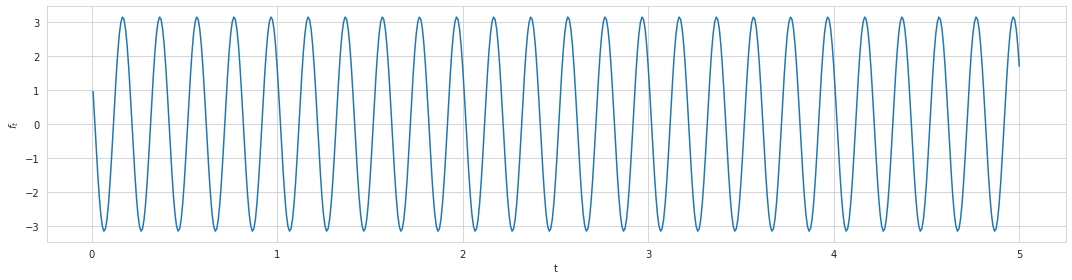
\includegraphics[width=0.9\textwidth]{plot1.png}
  \captionsetup{justification=centering}
  \caption{ACF & PACF plots}
\end{figure*}


\end{document}